\documentclass[notes,polish,xcolor=dvipsnames,hyperref={unicode,hidelinks,pdftex,pdfauthor={Patryk Bęza},pdftitle={Protokół zarządzania stacjami komputerowymi pod kontrolą systemu Linux},pdfsubject={Praca dyplomowa magisterska na Wydziale Matematyki i Nauk Informacyjnych Politechniki Warszawskiej},pdfkeywords={Software Configuration Management, SCM, Infrastructure as Code, IaC, Linux, Communications Protocol},pdfproducer={XeLaTeX},pdfcreator={latexmk}}]{beamer}
%\documentclass[notes,polish,xcolor=dvipsnames,aspectratio=169,hyperref={unicode,hidelinks,pdftex,pdfauthor={Patryk Bęza},pdftitle={Protokół zarządzania stacjami komputerowymi pod kontrolą systemu Linux},pdfsubject={Praca dyplomowa magisterska na Wydziale Matematyki i Nauk Informacyjnych Politechniki Warszawskiej},pdfkeywords={Software Configuration Management, SCM, Infrastructure as Code, IaC, Linux, Communications Protocol},pdfproducer={XeLaTeX},pdfcreator={latexmk}}]{beamer}             % wygenerować prezentację również w tym formacie

%\usefonttheme{professionalfonts} % using non standard fonts for beamer
%\usefonttheme{serif} % default family is serif
%\usepackage{fontspec}
%\setmainfont{Liberation Serif}

\usetheme{Rochester}
\usepackage[polish]{babel}
\usepackage{xcolor}
\definecolor{UniBlue}{RGB}{0,103,148}
\setbeamercolor{structure}{fg=UniBlue}
%\documentclass[notes=only]{beamer}			% only notes
%\setbeamertemplate{note page}[plain]
%\usefonttheme[onlymath]{serif}
%\usepackage[OT4,plmath]{polski}
\usepackage[utf8]{inputenc}
%\usepackage[polish]{translator}                        % https://tex.stackexchange.com/q/62185/44382
\usepackage[T1,plmath]{polski}
\usepackage{booktabs}
%\usepackage{enumitem}
%\usepackage{graphicx}                                  % loaded implicitly by Beamer
\usepackage{breakurl}
%\usepackage{hyperref}
%\usepackage[hyphens]{url}
\usepackage{lmodern}
\usepackage{multimedia}
\usepackage{pgfpages}
%\usepackage{unicode-math}
\usepackage{wrapfig}
\usepackage{mathtools}
%\usepackage[compatibility=false]{caption}
\usepackage{float}
\usepackage[caption=false]{subfig}
\usepackage{listings}
\usepackage{fancyvrb}
\usepackage{bytefield}
\usepackage{array}
\usepackage[none]{hyphenat}
\usepackage{tabto}
\usepackage{textcomp}
\usepackage{tikz}
\usetikzlibrary{arrows,automata}
\usepackage[absolute,overlay]{textpos}                   % podpisy autorów obrazków
\usepackage{adjustbox}

%\beamertemplatenavigationsymbolsempty
\DeclarePairedDelimiter{\ceil}{\lceil}{\rceil}

\newcommand{\smalllogoheight}{1.1cm}

\setbeamercolor*{block title example}{bg=blue!14}
\setbeamercolor*{block body example}{bg=blue!5}

%------------------------------------------------------------------------------
% Strona tytułowa
%------------------------------------------------------------------------------

\title{Protokół zarządzania stacjami komputerowymi\\pod~kontrolą systemu Linux}
\subtitle{[~Management Protocol for Linux Workstations~]}
\author[P.Bęza]{Patryk Bęza}
\institute[MiNI PW]{
	\vspace*{-7pt}\\
	Promotor: dr~inż.~Marek~Kozłowski\\[3pt]
	Wydział Matematyki i~Nauk Informacyjnych\\
	Politechnika Warszawska\\[12pt]
	\begin{tikzpicture}[remember picture,overlay]
		\node {
\includegraphics[height=\smalllogoheight]{img/mini}};%
	\end{tikzpicture}\hspace{40pt}
	\begin{tikzpicture}[remember picture,overlay]
		\node {
\includegraphics[height=\smalllogoheight]{img/pw}};%
	\end{tikzpicture}\\[6pt]
}
\date{\today}

% Obrazek na stronie tytułowej

%\titlegraphic{\hspace*{1em}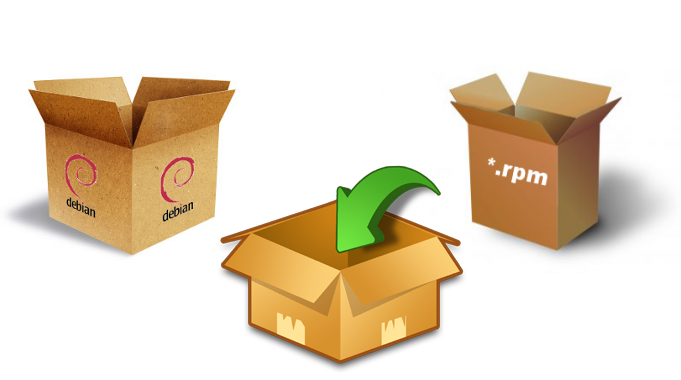
\includegraphics[height=.22\textheight]{img/package-manager}}

% Logo MiNI i PW na górze slajdu tytułowego

\addtobeamertemplate{title page}{}{%
	\newcommand{\titlepagelogoheight}{1.33cm}
	\begin{tikzpicture}[remember picture,overlay]
	\node[anchor=north west,yshift=0pt,xshift=3pt] at (current page.north west) {\includegraphics[height=\titlepagelogoheight]{img/mini-white}};%
	\node[anchor=north west,yshift=0pt,xshift=3pt] at (current page.north west) {\includegraphics[height=\titlepagelogoheight]{img/mini-white}};%
	\node[anchor=north east,yshift=0pt,xshift=-3pt] at (current page.north east) {\includegraphics[height=\titlepagelogoheight]{img/pw-white}};%
	\node[anchor=north east,yshift=0pt,xshift=-3pt] at (current page.north east) {\includegraphics[height=\titlepagelogoheight]{img/pw-white}};%
\end{tikzpicture}}

% Logo MiNI i PW w prawym górnym rogu slajdów (https://tex.stackexchange.com/q/27906/44382)

\addtobeamertemplate{frametitle}{}{%
	\newcommand{\frametitlelogoheight}{1.2cm}
	\begin{tikzpicture}[remember picture,overlay]
	\node[anchor=north east,yshift=0pt,xshift=-3pt] at (current page.north east) {\includegraphics[height=\frametitlelogoheight]{img/pw-white}};%
	\node[anchor=north east,yshift=0pt,xshift=-3pt] at (current page.north east) {\includegraphics[height=\frametitlelogoheight]{img/pw-white}};%
	\node[anchor=north east,yshift=-1pt,xshift=-45pt] at (current page.north east) {\includegraphics[height=\frametitlelogoheight]{img/mini-white}};%
	\node[anchor=north east,yshift=-1pt,xshift=-45pt] at (current page.north east) {\includegraphics[height=\frametitlelogoheight]{img/mini-white}};%
\end{tikzpicture}}

% Usunięcie przycisków nawigacji prezentacji

\setbeamertemplate{navigation symbols}{}

% Obrazek przy spisie treści
% https://tex.stackexchange.com/a/392822/44382

\DeclareRobustCommand\PICINTOC{}%
\newcommand\MYPICINTOC{\hfill\smash{\raisebox{-1.2\height}{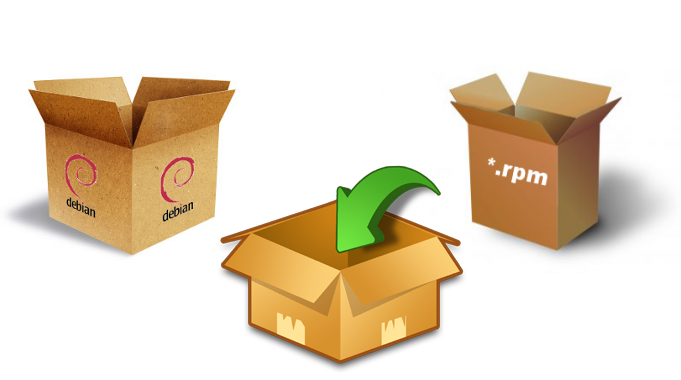
\includegraphics[width=.38\textwidth]{img/package-manager}}}}

\begin{document}

%------------------------------------------------------------------------------

\begin{frame}

\titlepage

\end{frame}

%------------------------------------------------------------------------------

\begin{frame}{Spis treści}

\addtocontents{toc}{\let\PICINTOC\string\MYPICINTOC}
\tableofcontents

\end{frame}

%------------------------------------------------------------------------------

\section{Problem, temat i~cel pracy\PICINTOC}

%------------------------------------------------------------------------------

\begin{frame}{Problem}

\vspace*{-0.5cm}
%\begin{center}
%\begin{minipage}{10.7cm}
\begin{exampleblock}{}
\textbf{Problem dystrybuowania ujednoliconego oprogramowania} do~dużej ilości maszyn roboczych pracujących pod kontrolą systemu \texttt{Linux}.
\end{exampleblock}
%\end{minipage}
%\end{center}

\vfill

\begin{itemize}
	\item Kogo dotyka problem?
	\item Miejsca zastosowania rozwiązania problemu
	\item ,,Ręczne'' metody radzenia sobie z~problemem
\end{itemize}

\vfill

\begin{center}
	\begin{minipage}{0.74\textheight}
		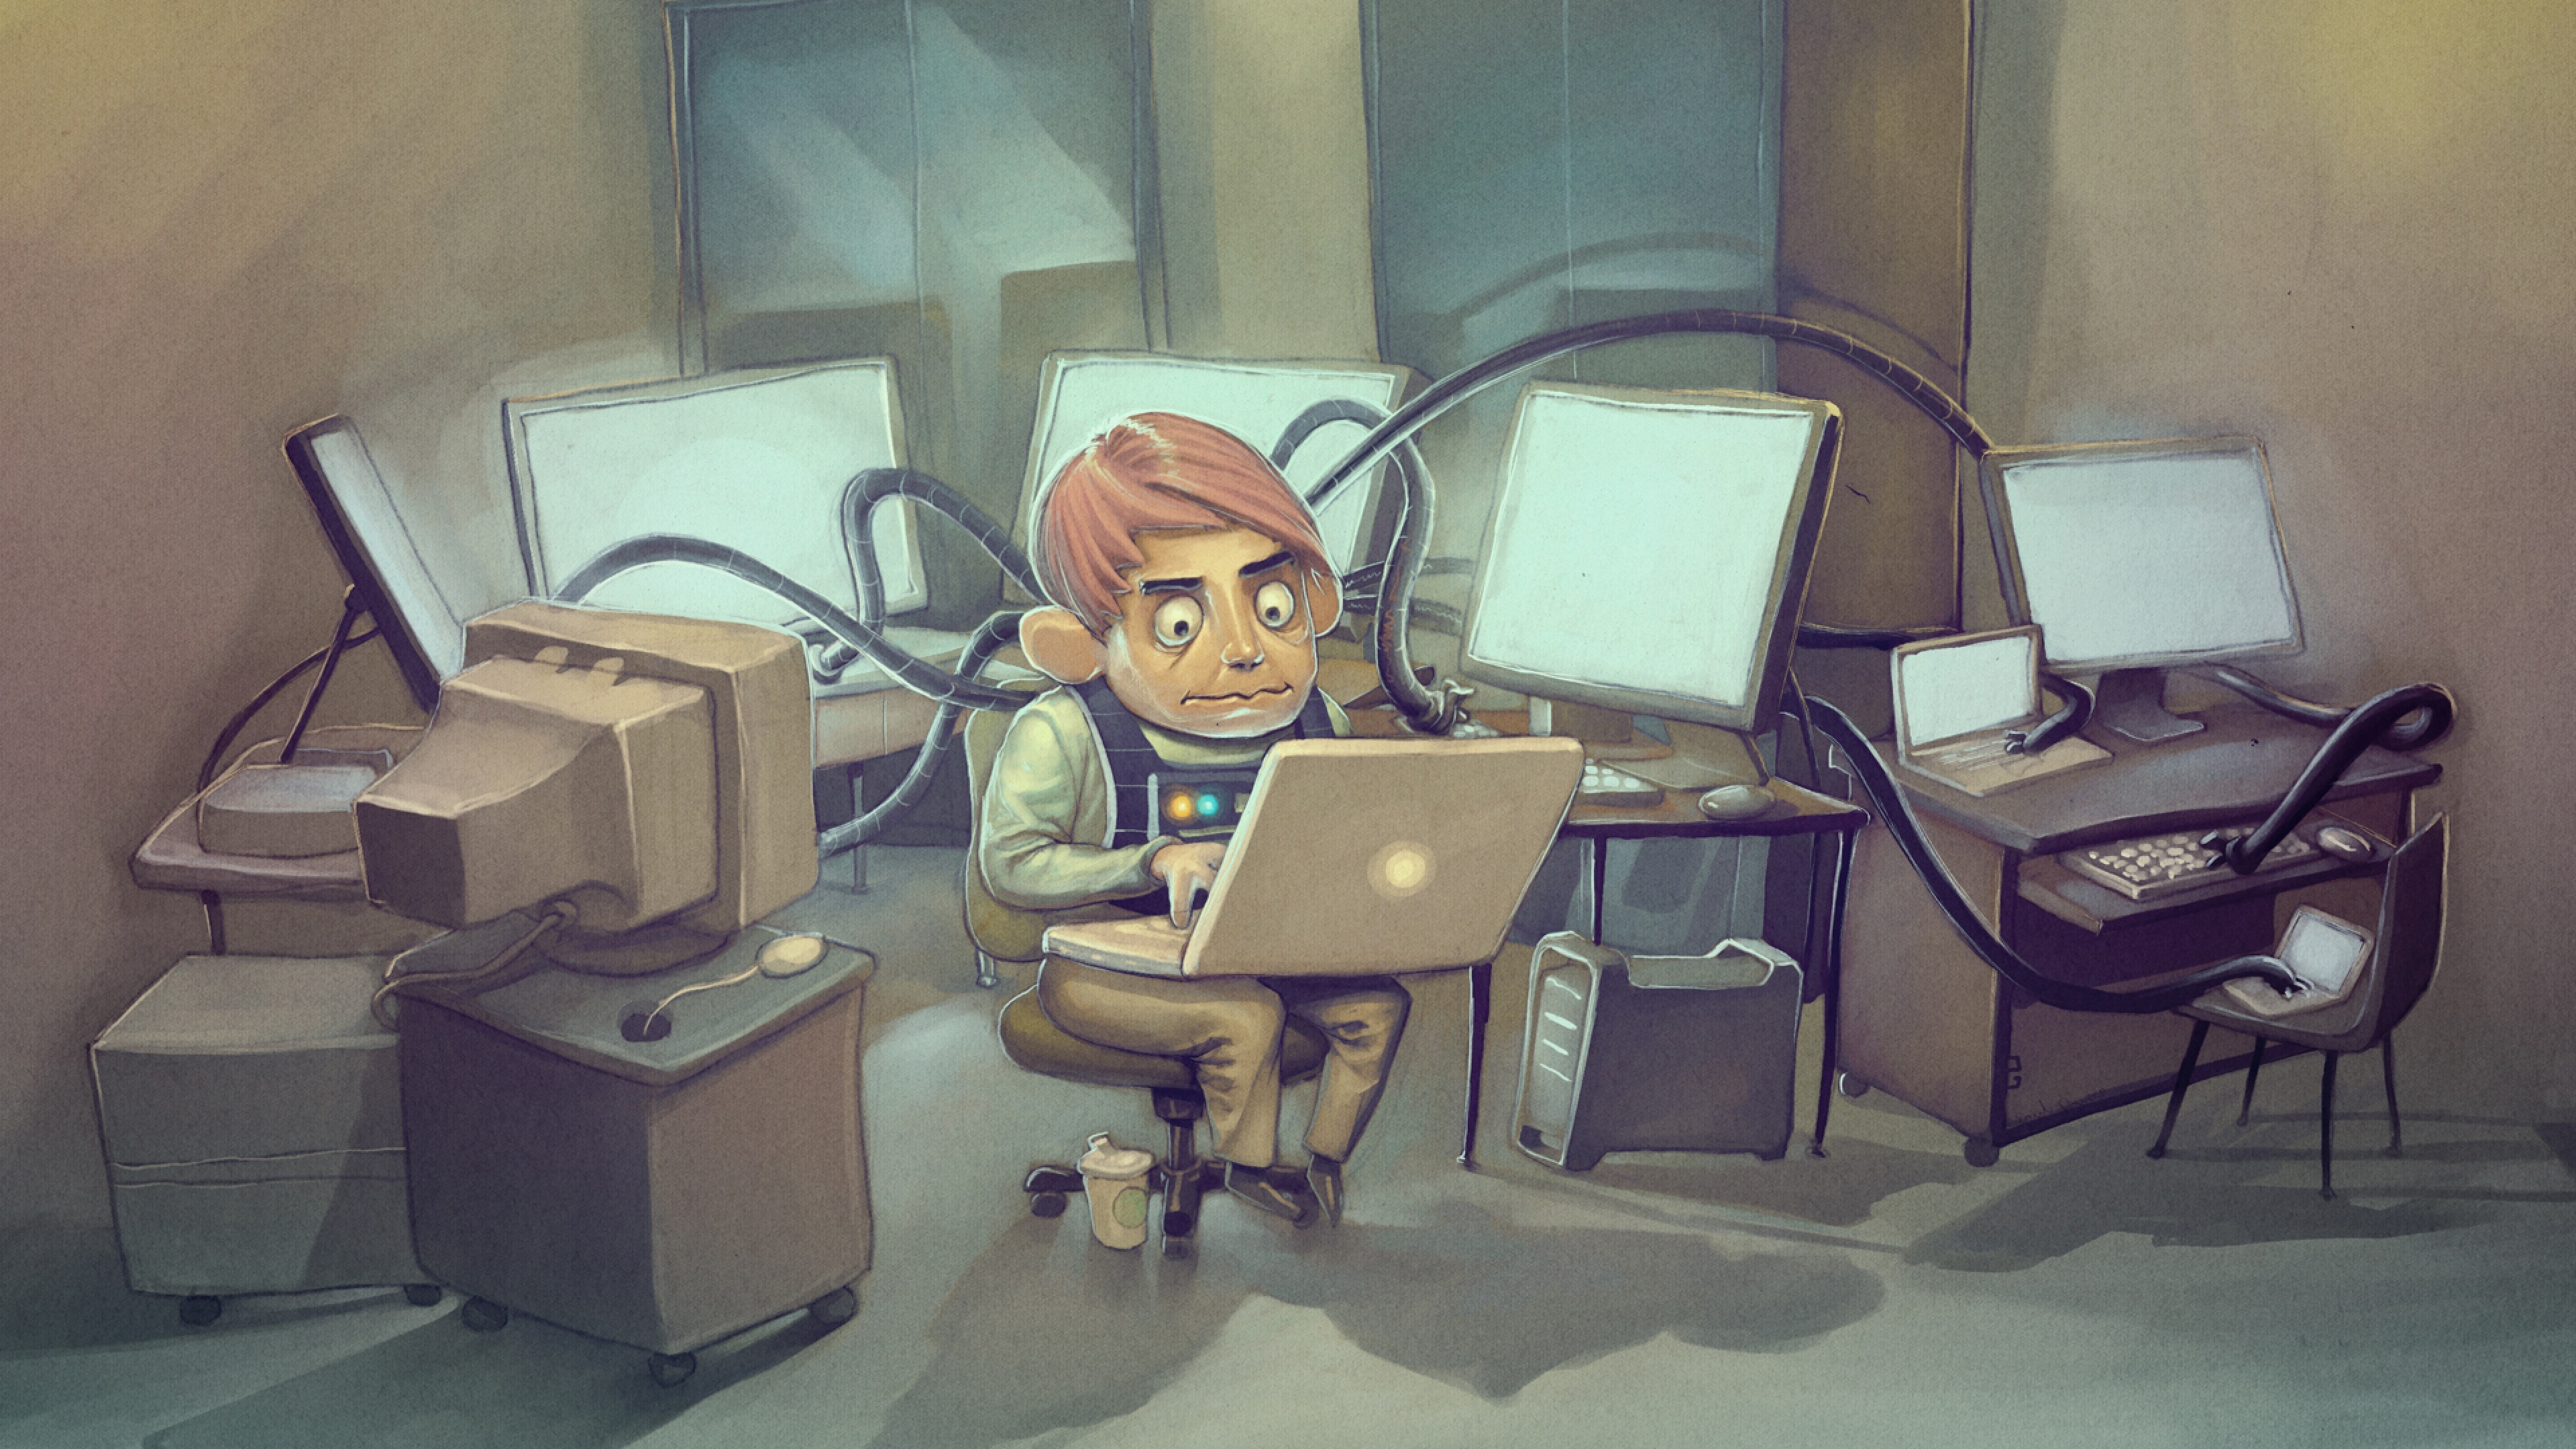
\includegraphics[width=\linewidth]{img/busy-admin}\\
		\raggedleft\color{gray}\tiny Źródło: \emph{virtuallnk.com (za zgodą sales@virtuallnk.com)}
	\end{minipage}
\end{center}

\end{frame}

\note[itemize]{
	\item \textbf{Przedstawienie problemu, którego dotyczy praca} i~zwrócenie uwagi na to, że~oprogramowanie na~konfigurowanych systemach nie musi być identyczne (szablony konfiguracji).
	\item \textbf{Kogo dotyczy problem?} Głównie administratorów komputerowych, ale też ludzi używających na~co~dzień wielu podobnie skonfigurowanych komputerów.
	\item \textbf{Gdzie można znaleźć zastosowania rozwiązania tego problemu?} Wszędzie tam gdzie działa grupa podobnie skonfigurowanych maszyn, np.: komputery w~laboratoriach na~uczelniach, szkołach, bibliotekach, urzędach, sklepach, grupy serwerów, biletomaty, bankomaty, automaty sprzedające (maszyny \emph{vendingowe}), komputery osób korzystających z~wielu komputerów.
	\item \textbf{Jakie są ,,ręczne'' metody radzenia sobie z~tym problemem bez wykorzystania dedykowanego oprogramowania?}\\,,Ręczna'' instalacja gotowego obrazu systemu na każdym z~komputerów, SSH, zdalny pulpit~(VNC).
}

%------------------------------------------------------------------------------

\begin{frame}{Temat i~cel pracy}

\begin{exampleblock}{}
	{\textbf{Zaprojektowanie i~zaimplementowanie protokołu} umożliwiającego \textbf{propagowanie zmian w~systemie plików, pakietów oraz~elementów konfiguracji} do~stacji roboczych pod~kontrolą systemu operacyjnego \texttt{GNU/Linux} lub~innego systemu \texttt{*nix}, a~także elastycznego standardu opisu zmian oraz~narzędzi dla~ich rejestrowania i~dostosowywania.}
	\vskip2mm
	\hspace*\fill{\small--- Formalnie zgłoszona tematyka pracy magisterski}
\end{exampleblock}

\begin{figure}
	\includegraphics[height=.32\textheight]{img/client_server}
\end{figure}

\end{frame}

\note[itemize]{
\item \textbf{Przeczytanie formalnie zgłoszonego do~Dziekanatu celu pracy.} Zwrócenie uwagi na, to, że~wbrew nazwie ,,protokół'' użytej w~tytule pracy, głównym celem było zaimplementowanie aplikacji ,,serwera'', która umożliwia przygotowanie i~dostosowanie obrazu zmian konfiguracji systemu wzorcowego, który można zastosować na~systemie klienckim za~pomocą aplikacji ,,klienckiej'', a~nie samo przesłanie takiego obrazu do~klienta (co~zostało zaimplementowane za~pomocą \texttt{SFTP}).
\item \textbf{Zwrócenie uwagi, że~przez serwer rozumie się stację ze~wzorcem oprogramowania dla~klientów}, a~nie klasyczny model komunikacji klient--serwer. Przyjęty model komunikacji działa raczej w~modelu \emph{peer2peer}.
\item Zwrócenie uwagi na~obsługę różnych systemów \texttt{GNU/Linux} i~na~to, że~zaimplementowane \textbf{rozwiązanie było testowane na~dystrybucjach \texttt{Debian} i~\texttt{ArchLinux}, ale~jest napisane w~języku Python i~prawdopodobnie działa również na~innych dystrybucjach.}
}

%------------------------------------------------------------------------------

\section{Istniejące rozwiązania}

\begin{frame}[fragile]{Istniejące rozwiązania --- systemy SCM}

\newcommand{\tablelogoheight}{0.71cm}
\newcommand*{\centerheader}[1]{\multicolumn{1}{c|}{\includegraphics[height=\tablelogoheight]{#1}}}
\newcommand{\puppetlogo}{\centerheader{img/Puppet_logo}}
\newcommand{\saltlogo}{\centerheader{img/SaltStack_logo}}
\newcommand{\ansiblelogo}{\centerheader{img/Ansible_logo}}
\newcommand{\cheflogo}{\multicolumn{1}{c}{
\includegraphics[height=\tablelogoheight]{img/Chef_logo}}}
\newcommand{\fixedcell}[1]{\parbox[l][0.52cm][c]{1.8cm}{\raggedleft #1}}
\renewcommand{\arraystretch}{1.7}
\newcolumntype{M}[1]{>{\centering\arraybackslash}m{#1}}
\newcolumntype{L}[1]{>{\raggedright\arraybackslash}m{#1}}
\newcolumntype{N}{@{}m{0pt}@{}}

\renewcommand*{\thefootnote}{\fnsymbol{footnote}} % gwiazdka zamiast numeracji arabskiej w przypisach
\setbeamerfont{footnote}{size=\tiny} % wielkość czcionki przypisów
\newcommand{\popularity}{miejsce w~rankingu popularności\footnote{Popularność wg liczby pobrań w~\emph{Debian Popularity Contest} (stan na~dzień 08.11.2017). W~nawiasach podano miejsce w~rankingu względem 3~pozostałych rozwiązań.}}

\begin{adjustbox}{center}
	\tiny
	\begin{tabular}{L{1.8cm}|M{2cm}|M{2cm}|M{2cm}|M{2cm}N}
		                               & \puppetlogo               & \ansiblelogo             & \saltlogo                      & \cheflogo                       \\\hline\hline
		\fixedcell{rok założenia}      & 2005                      & 2012                     & 2011                           & 2009                            \\\hline
		\fixedcell{język}              & Ruby                      & Python, PowerShell       & Python                         & Ruby, Erlang                    \\\hline
		\fixedcell{model}              & klient-serwer             & tylko serwer             & klient-serwer lub~tylko serwer & klient-serwer                   \\\hline
		\fixedcell{plik konfiguracji}  & \emph{manifest}           & \emph{playbook}          & ---                            & \emph{recipe} / \emph{cookbook} \\\hline
		\fixedcell{znani użytkownicy}  & CERN, Google, NASA, Intel & Apple, NASA, Juniper     & LinkedIn, TD~Bank              & Facebook, IBM, HP, Mozilla      \\\hline
		\fixedcell{licencja}           & Apache~2.0                & GPLv3                    & Apache~2.0                     & Apache~2.0                      \\\hline
		\fixedcell{założyciel}         & Luke Kanies (USA,~OR)     & Michael Dehaan (USA,~NC) & Thomas Hatch (USA,~UT)         & Adam Jacob (USA,~WA)            \\\hline
		\fixedcell{\popularity}        & 6061 (1)                  & 8547 (2)                 & 8796 (3)                       & 12675 (4)
% Deklaratywny język konfiguracji wszystkich rozwiązań (nie imperatywny)
	\end{tabular}
\end{adjustbox}
\vfill

\end{frame}

\note[itemize]{
	\item \textbf{Wyjaśnienie, że~rozwiązaniem przedstawionego problemu są~systemy nazywane systemami SCM, czyli \emph{Software Configuration Systems}} --- nie mylić z~oprogramowaniem typu \emph{Source Control Management}, takimi jak np.~\texttt{git} i~\texttt{svn}.
	\item \textbf{Scharakteryzowanie 4 (prawdopodobnie jednych z~najpopularniejszych) systemów zarządzania konfiguracją opisanych w~pracy.} Zwrócenie uwagi na~duże firmy i~instytucje używające tego wymienionych rozwiązań (CERN, NASA, Google~itd.).
	\item \textbf{Deklaratywna konfiguracja przedstawionych rozwiązań (a~nie imperatywna).}
	\item \textbf{Wyróżnienie Puppet pod~względem wyrafinowania i~popularności (vide ranking).} Wyrafinowanie polega na~budowaniu grafu zależności zasobów i~decydowanie na~jego podstawie w~jakiej kolejności zmieniać konfigurację systemu.
}

%------------------------------------------------------------------------------

\section{Własne rozwiązanie problemu}

\begin{frame}{Alternatywne rozwiązanie problemu}

Sposób wykorzystania alternatywnego rozwiązania:
\begin{itemize}
	\item \textbf{Skanowanie} systemu wzorcowego
	\item \textbf{Modyfikacja} konfiguracji i~oprogramowania systemu wzorcowego
	\item Ponowne \textbf{skanowanie} systemu wzorcowego
	\item \textbf{Generowanie obrazu} zmian konfiguracji systemu wzorcowego na~podstawie ostatniego skanowania i~wybranego
	\item \textbf{Pobranie i~zastosowanie obrazu} zmian konfiguracji przez klienta
\end{itemize}

\begin{figure}
	\centering
	\begin{tikzpicture}[>=latex',shorten >=1pt,auto,node distance=3.1cm]
		\node[state,ultra thick] (q0)               {};
		\node[state,ultra thick] (q1) [right of=q0] {};

		\path[->] (q0) edge[very thick,font=\scriptsize,bend left] node[align=center] {skanowanie\\systemu}  (q1);
		\path[->] (q1) edge[very thick,font=\scriptsize,bend left]  node[align=center] {zmiany\\konfiguracji} (q0);
		\path[->] (q1) edge[very thick,font=\scriptsize,loop right] node[align=center] {tworzenie\\obrazu zmian\\konfiguracji} (q1);
	\end{tikzpicture}
\end{figure}

\end{frame}

\note{\textbf{Zupełnie inne podejście w~porównaniu do~istniejących rozwiązań} --- zamiast deklaratywnie/imperatywnie opisywać oczekiwany stan systemu wystarczy skonfigurować maszynę wzorcową.}

%------------------------------------------------------------------------------

\begin{frame}{Alternatywne rozwiązanie problemu cd.}

Cechy rozwiązania:
\begin{itemize}
	\item \textbf{Łatwość użytkowania} --- brak potrzeby pisania reguł określających pożądaną konfigurację klientów i~nauki języka w~którym byłyby one wyrażone
	\item \textbf{Rozproszenie} --- rozproszony model dzielenia się konfiguracją systemu wzorcowego
	\item \textbf{Wykorzystanie szablonów} --- parametryzacja konfiguracji np.~zmiennymi środowiskowymi
	\item \textbf{Uniwersalność} --- obsługa różnych dystrybucji \texttt{Linux}
	\item \textbf{Bezpieczeństwo} --- konfiguracja systemu wzorcowego podpisana cyfrowo
	\item \textbf{Elastyczność} --- możliwość synchronizacji części konfiguracji
\end{itemize}

\end{frame}

%------------------------------------------------------------------------------

\section{Implementacja}

\begin{frame}{Implementacja}

\begin{itemize}
	\item 3 moduły: \texttt{myscm-srv}, \texttt{myscm-cli} i~\texttt{myscm-common}
	\item Początkowo w~języku~\texttt{C}, ostatecznie w~\textbf{\texttt{Python~3}}
	\item Przetestowana obsługa dystrybucjach \textbf{\texttt{Arch Linux}} i~\textbf{\texttt{Debian}}
	\item Wykorzystanie m.in.~\textbf{\texttt{AIDE}} i~\textbf{\texttt{OpenSSL}}
\end{itemize}

\end{frame}

\note[itemize]{
	\item Napomknienie o~tym, że~na~początku planowałem zaimplementować całe rozwiązanie w~języku \texttt{C}, ale~okazało się, że~dużo łatwiej było wykorzystać język wysokopoziomowy (jakim jest np.~\texttt{Python})
	\item Wszystkie wspomniane \textbf{istniejące rozwiązania są~w~językach wysokopoziomowych} (poza \emph{CFEngine} wspomnianym w~pracy)
}

%------------------------------------------------------------------------------

\begin{frame}{Testy}

\begin{itemize}
	\item \textbf{Trudność automatyzacji testów}
	\item \textbf{,,Małe'' testy} --- półautomatyczne, wykonywane regularnie na~niewielkim drzewie plików
	\item \textbf{,,Duże'' testy} --- manualne, wykonane pod~koniec projektu na~pełnym systemie operacyjnym
	\item \textbf{Synchronizowane katalogi}: \path{/bin}, \path{/etc}, \path{/lib}, \path{/lib64}, \path{/sbin}, \path{/srv}, \path{/usr}, \path{/var/lib/dpkg} (\path{/var/lib/pacman})
	\item \textbf{Niesynchronizowane katalogi}: \path{/boot}, \path{/dev}, \path{/home}, \path{/lost+found}, \path{/media}, \path{/mnt}, \path{/opt}, \path{/proc}, \path{/root}, \path{/run}, \path{/sys}, \path{/tmp} i~\path{/var} (poza~ww.)
	\item \textbf{Błędy} po~pierwszych ,,dużych'' testach:
		\begin{itemize}
			\item \textbf{pliki binarne} \path{/etc/ld.so.cache}, \path{/etc/localtime} w~katalogu \path{/etc}
			\item \textbf{,,nietypowe'' znaki} w~ścieżkach pliku (np.~dwukropka)
			\item \textbf{niesynchronizowanie \path{/var/lib/lightdm}}
		\end{itemize}
\end{itemize}

\end{frame}

\note[itemize]{
\item Zwrócenie uwagi na to, że~w~trakcie implementacji działanie programu było testowane na~stosunkowo \textbf{niewielkim drzewie plików (,,małe'' testy)}.
\item \textbf{,,Duże'' testy} odbyły się \textbf{na~koniec projektu na~dwóch pełnych systemach} i~zakończyły się wykryciem kilku drobnych błędów, które zostały naprawione, a~testy z~sukcesem powtórzone.
\item Wyjaśnienie wykrytych błędów i~dodanie, że:
	\begin{itemize}
	\item dla~wszystkich zmienionych plików w~\path{/etc} są~robione \textbf{różnice plików (''\texttt{diff-y}'')}, a~pliki binarne były tam nieprzewidziane,
	\item w~\texttt{Linux} (a~właściwie w~systemach plików \texttt{ext2-4}) \textbf{w~ścieżkach plików są~dozwolone wszystkie znaki poza lewym ukośnikiem (\texttt{\textbackslash}) i~znakiem \texttt{\textbackslash{}0} (\texttt{null byte})},
	\item niesynchronizowanie \path{/var/lib/lightdm} powodowało \textbf{nieuruchamianie się środowiska graficznego}, ale~była możliwa praca w~konsoli (jak w~\emph{runlevelu}~3).
	\end{itemize}
}

%------------------------------------------------------------------------------

\section{Dalsze możliwe kierunki rozwoju projektu}

\begin{frame}{Dalsze możliwe kierunki rozwoju}

\begin{itemize}
	\item \textbf{Dodanie obsługi innych protokołów wymiany plików} lub~zastąpienie \texttt{SFTP} protokołem \emph{multicastowym}
	\item \textbf{Obsługa kłopotliwych do~obsłużenia sytuacji} np.~podczas aktualizacji jądra systemu (\texttt{GRUB})
	\item Dodanie możliwości tworzenia obrazów zmian na~podstawie \textbf{dowolnych dwóch wyników skanowań} systemu wzorcowego
	\item \textbf{Lepsza obsługa sytuacji awaryjnych} --- np.~nagłe przerwanie procesu zastosowania obrazu zmian powinno być tranzakcyjne (wszystko albo nic)
	\item Dodanie możliwości opcjonalnego zdalnego \textbf{raportowania [nie]powodzenia} zastosowania obrazu zmian przez klientów
	\item Dodanie obsługi \textbf{innych systemów operacyjnych} niż~\texttt{Linux}
\end{itemize}

\end{frame}

%------------------------------------------------------------------------------

\section{Podsumowanie}

\begin{frame}{Podsumowanie}

\begin{itemize}
	\item \textbf{Zaimplementowano aplikację} przeznaczoną do~\textbf{tworzenia, dostosowywania i~zastosowania obrazów} zmian konfiguracji systemu wzorcowego dla~systemów \texttt{GNU/Linux}
	\item Zadbano o~bezpieczeństwo, a~konkretnie \textbf{autentyczność} (uwierzytelnienie) wygenerowanego obrazu zmian jest \textbf{podpis cyfrowy~SSL}
	\item Umożliwiono klientom \textbf{dzielenie się między sobą obrazami zmian konfiguracji}
	\item \textbf{Opisano 4~najpopularniejsze istniejące rozwiązania} i~wspomniano o~innych
	\item \textbf{Udokumentowano} sposób działania zaimplementowanej aplikacji (\LaTeX + dokumentacja w~kodzie źródłowym)
\end{itemize}

\end{frame}

%------------------------------------------------------------------------------

\begin{frame}{Koniec}

\begin{center}
	\LARGE Dziękuję za~uwagę\\[1em]
	\begin{minipage}{1.1\textheight}
		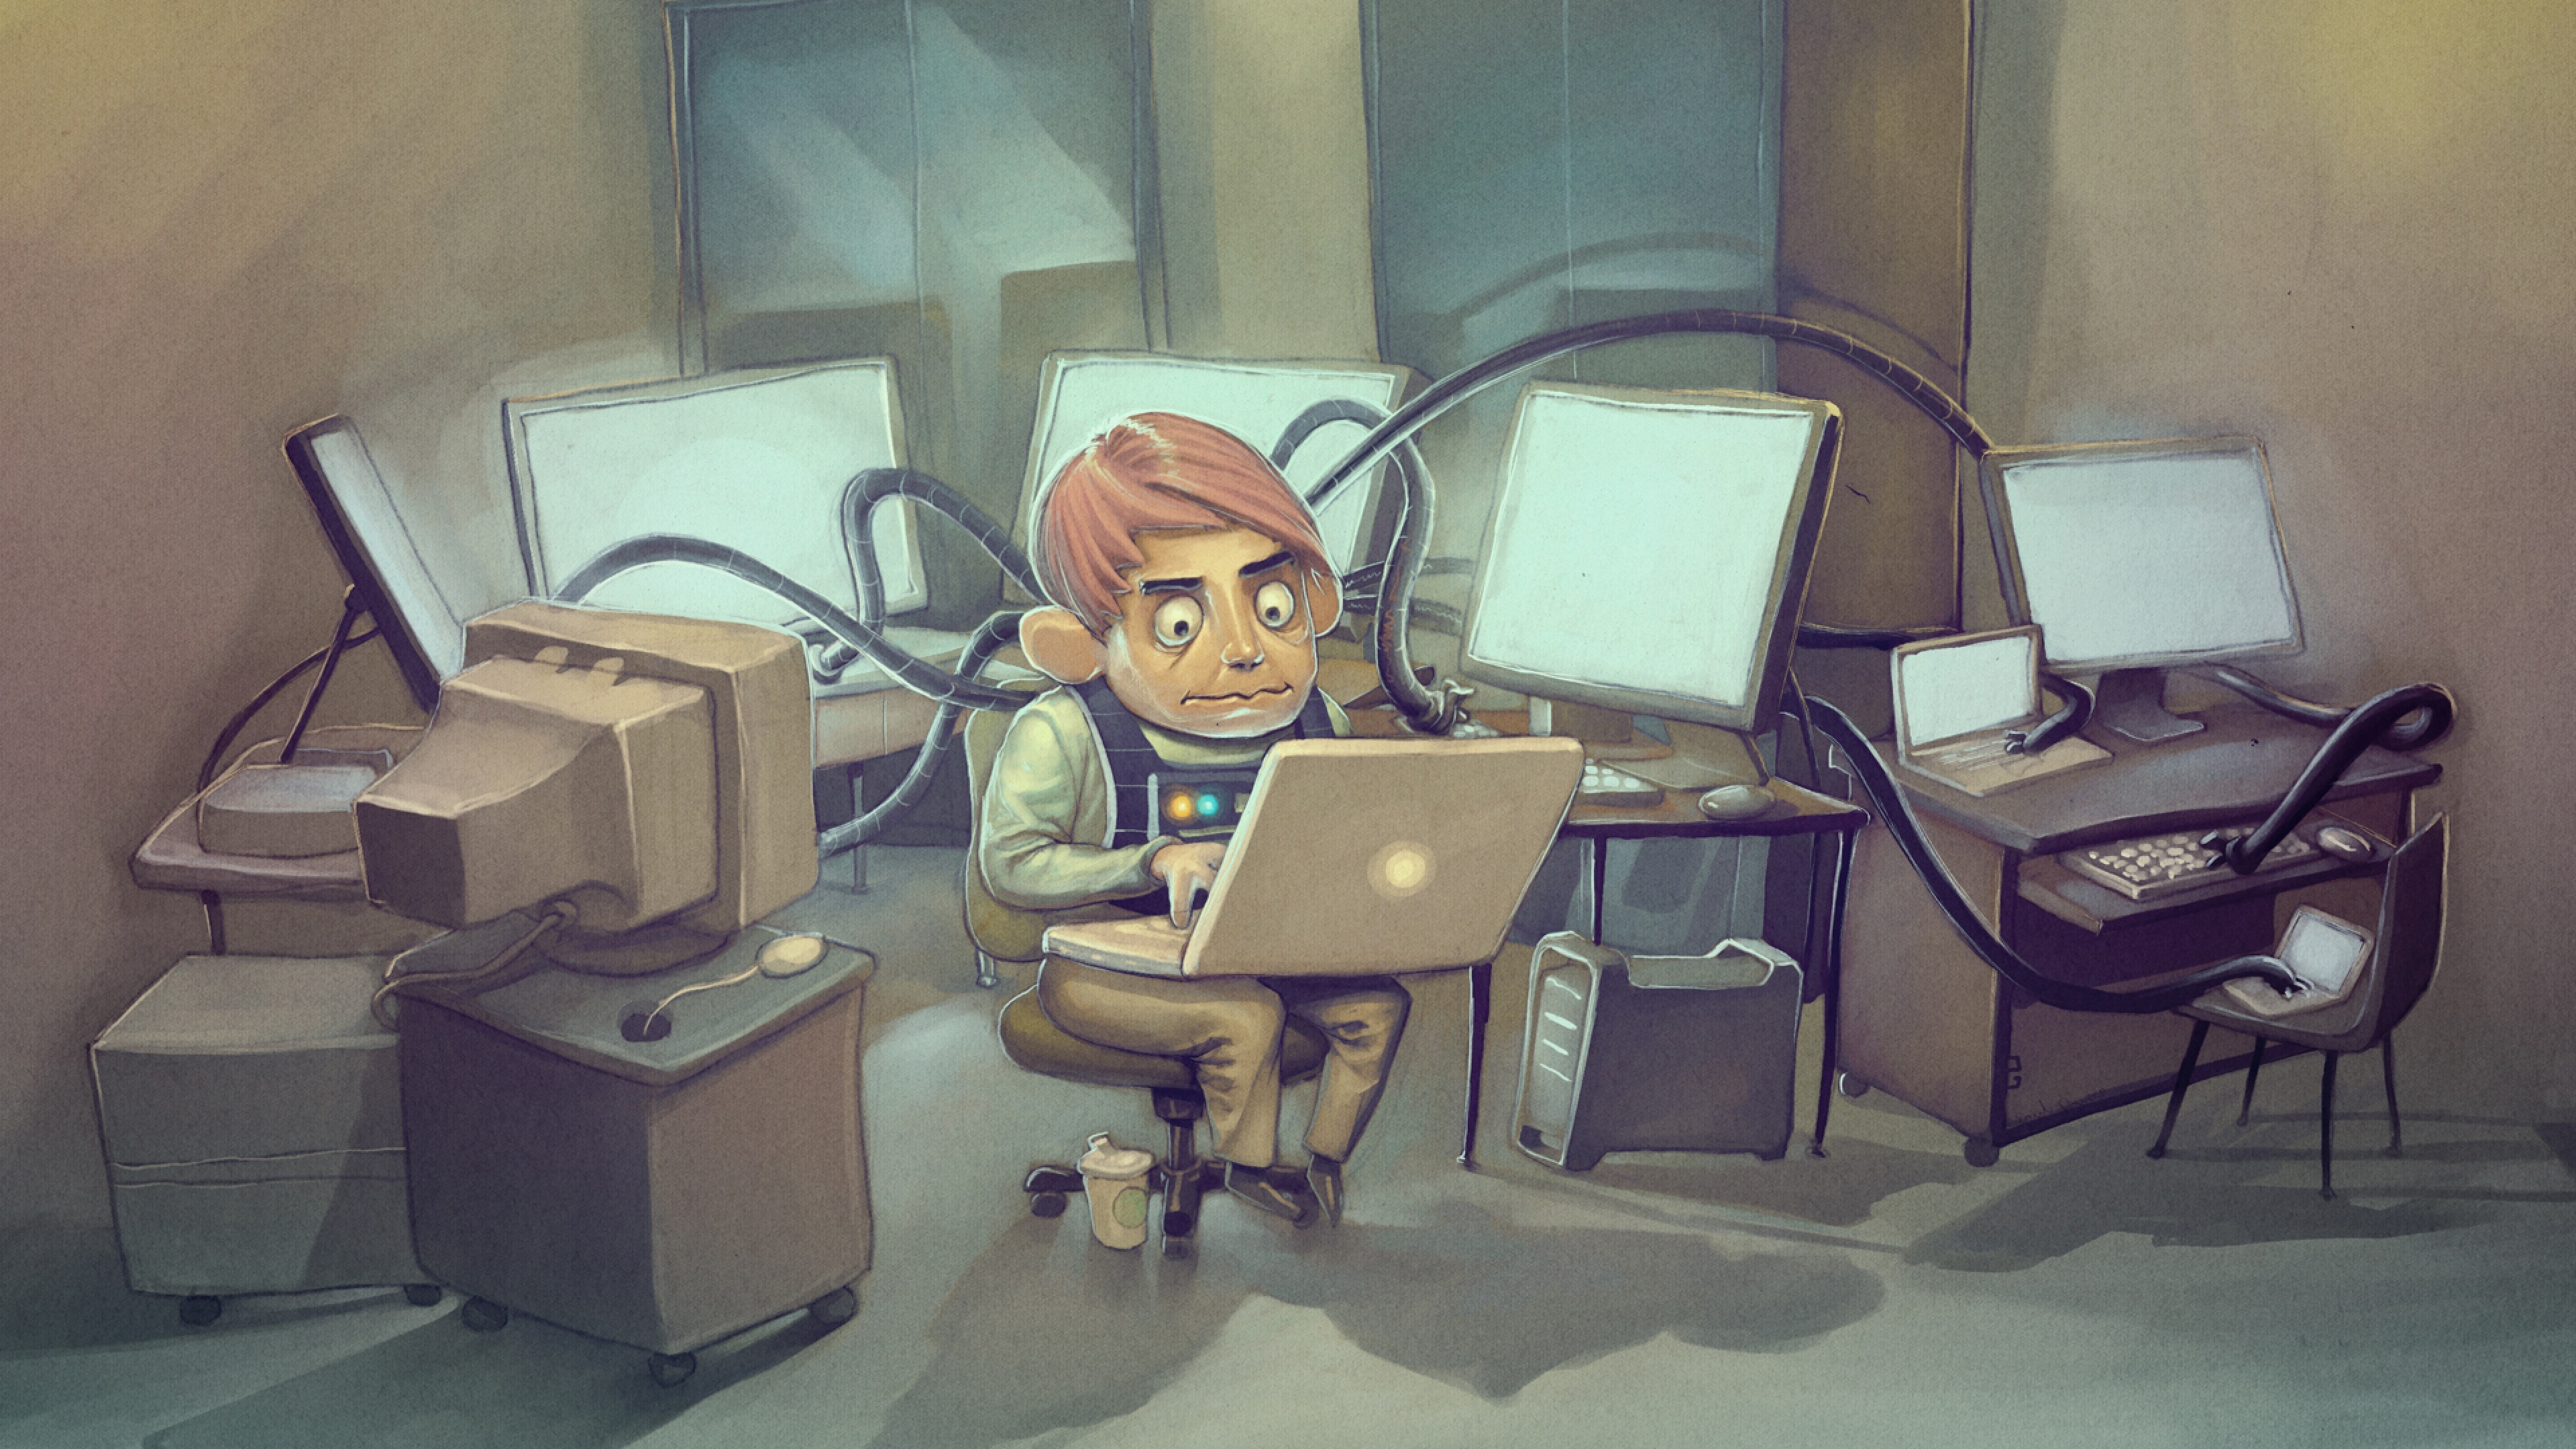
\includegraphics[width=\linewidth]{img/busy-admin}\\
		\raggedleft\color{gray}\tiny Źródło: \emph{virtuallnk.com (za zgodą sales@virtuallnk.com)}
	\end{minipage}
\end{center}

\end{frame}

%------------------------------------------------------------------------------

\end{document}
